\section{Theorie} \label{sec:theorie}

    Im Folgenden sollen die theoretischen Grundlagen der Wechselwirkung von Neutronen mit Kernen aufgeführt werden.

\subsection{Neutronen}

    In diesem Versuch werden die Neutronen durch die Reaktion von Berilium-Kernen mit $\alpha$-Teilchen erzeugt.
    \begin{equation*}
        \ce{^{9}_{4}Be + ^{4}_{2} \symup{\alpha} -> ^{12}_{6}C + ^{1}_{0}n}
    \end{equation*}
    Um die entstandenen Neutronen abzubremsen, da besonders die langsameren benötigt werden,
    werden sie durch Materieschichten, in diesem Fall Paraffin, gelenkt.
    Dabei kommt es zu elastischen Stößen mit den Atomen der Materie und die Neutronen geben Energie an leichtere Kerne ab.
    So entstehen thermische Neutronen,
    mit einer Energie von $\SI{0,025}{\electronvolt}$ bei einer Temperatur von $\SI{290}{\kelvin}$
    und einer mittleren Geschwindigkeit von $\SI{2,2}{\kilo\meter\per\second}$.

    \begin{figure}[H]
      \centering
      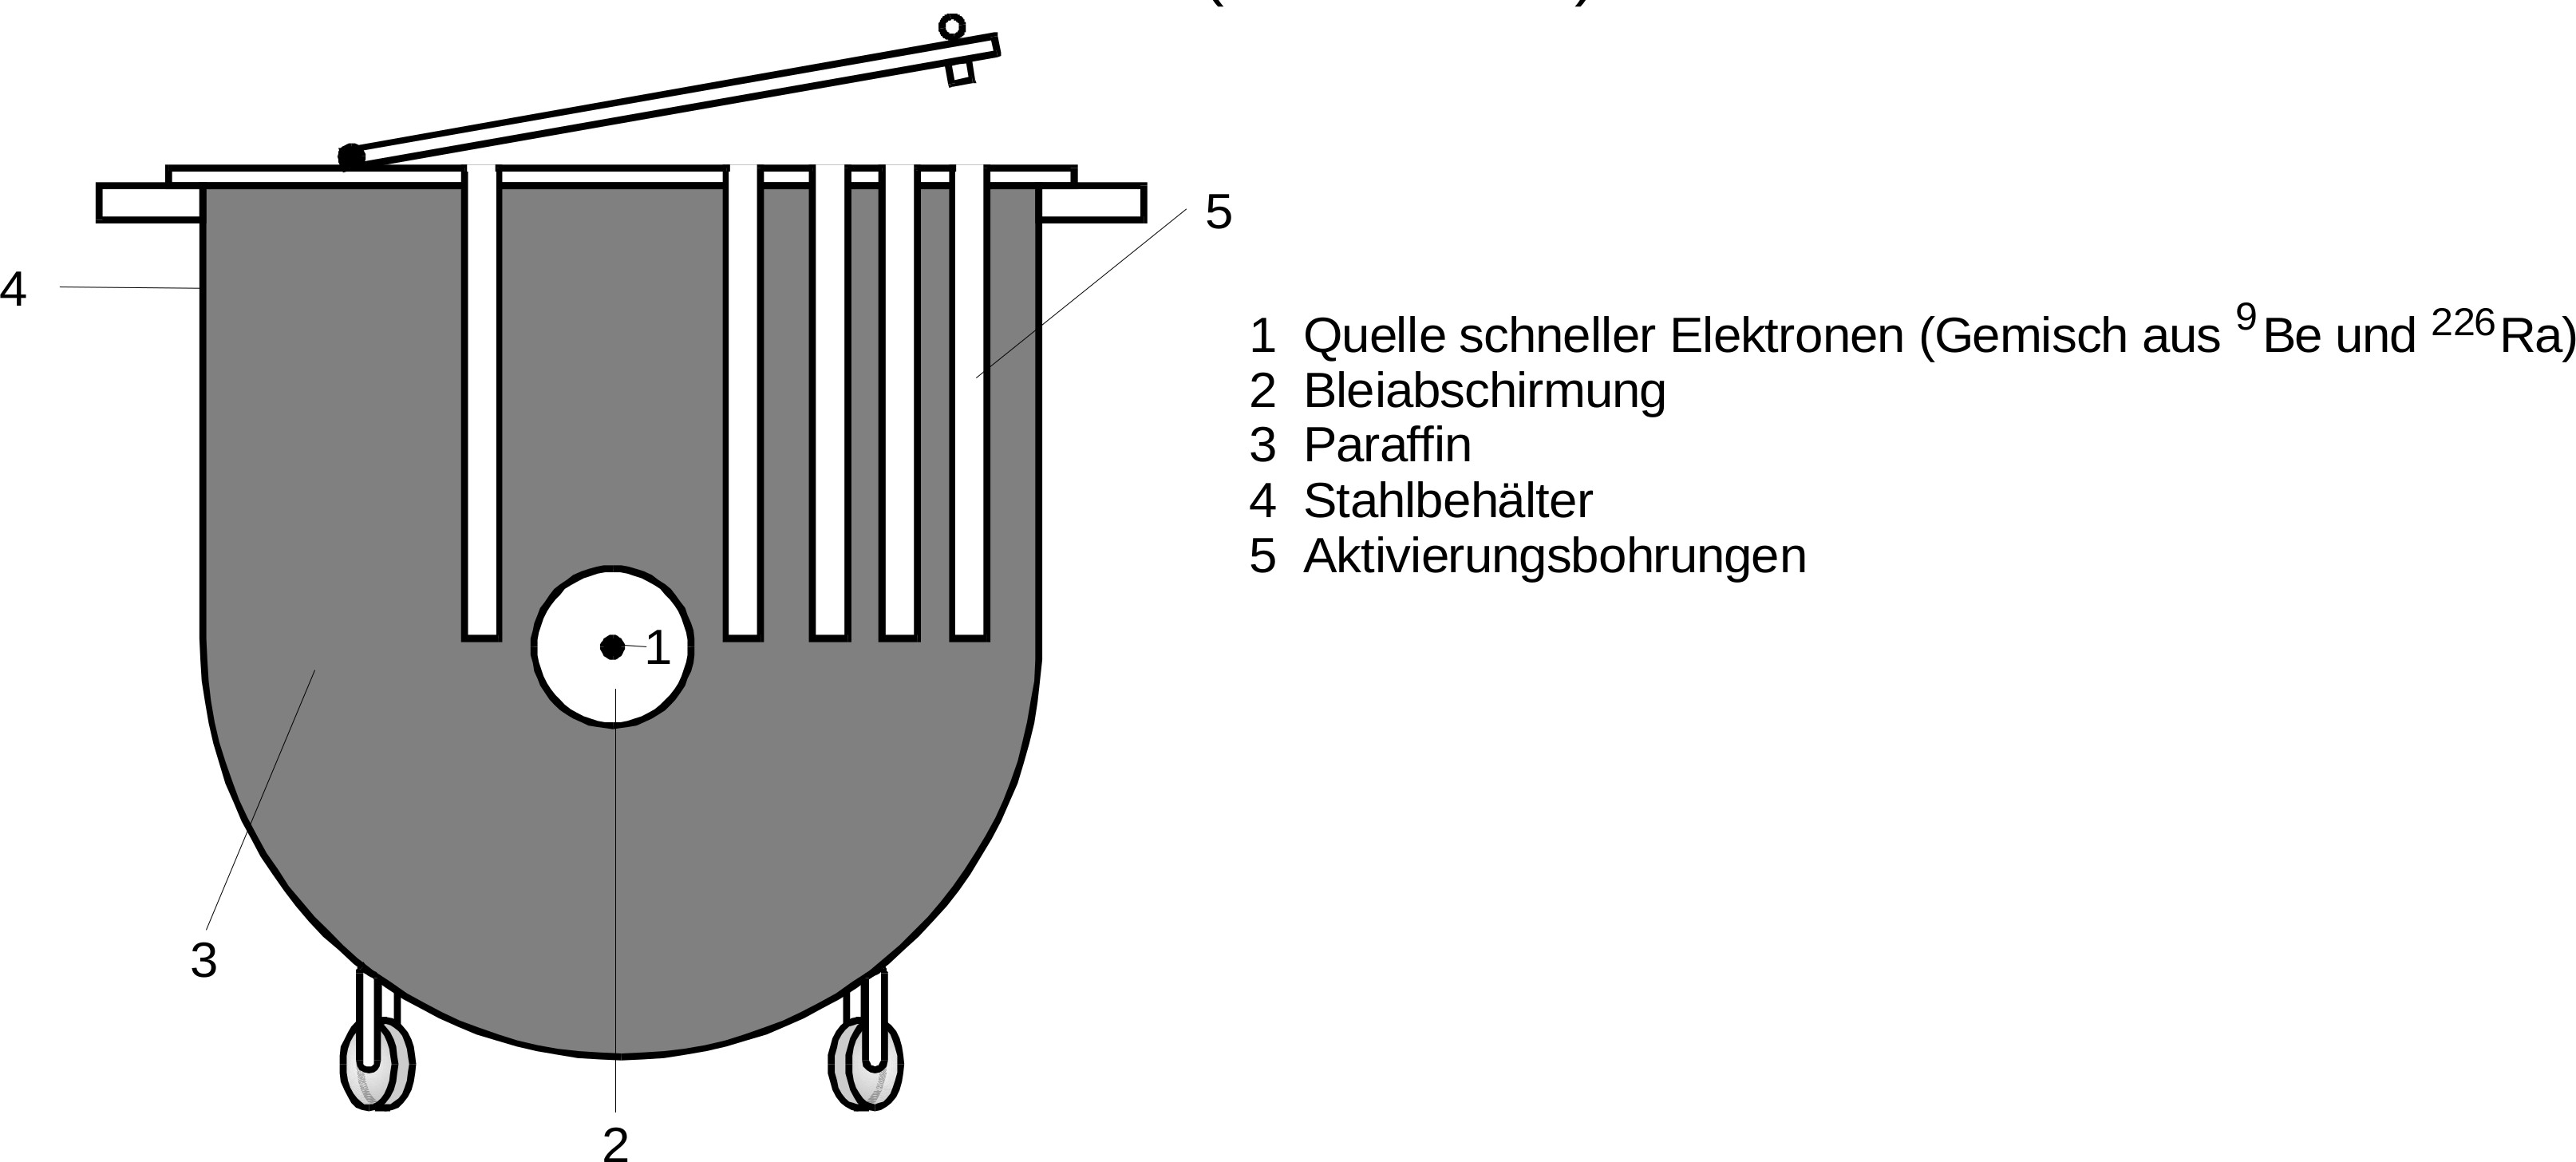
\includegraphics[width=\textwidth]{content/img/V702_Abb1.jpg}
      \caption{Querschnitt durch die hier verwendete Quelle für thermische Neutronen \cite{versuchsanleitung}.}
      \label{fig:neutronenquelle}
    \end{figure}

    Wenn nun ein Neutron auf einen Kern $\ce{A}$ trifft,
    wird es absorbiert, und es entsteht ein Zwischenkern $\ce{A^*}$ mit einer höhereren Energie. \\
    Die Wahrscheinlichkeit, mit der ein Neutron eingefangen wird,
    wird durch den Wirkungsquerschnitt $\sigma$ beschrieben,
    welcher antiproportional zur Geschwindigkeit der Neutronen ist.
    Je geringer also die Geschwindigkeit der Neutronen ist,
    desto höher ist die Wahrscheinlichkeit,
    dass ein Kern ein Neutron einfängt. \\
    Nach etwa $\SI{e-16}{\second}$ geht der Kern wieder in seinen Grundzustand über;
    die überschüssige Energie wird dabei in Form eines $\gamma$-Quants ausgestoßen.
    \begin{equation*}
        \ce{^{m}_{z}A + ^{1}_{0}n -> ^{m+1}_{z} A^* -> ^{m+1}_{z} A + \symup{\gamma}}
    \end{equation*}
    Aufgrund des zusätzlichen Neutrons ist der Zwischenkern allerdings nicht stabil,
    sondern zerfällt in einen stabilen Kern $\ce{^{m+1}_{z+1} C}$ unter Emission eines Elektrons und eines Elektronantineutrinos,
    auf die die überschüssige Masse des Kerns $\ce{^{m+1}_{z} A^*}$ in Form von kinetischer Energie aufgeteilt wird.
    \begin{equation*}
        \ce{^{m+1}_{z} A -> ^{m+1}_{z+1} C + \symup{\beta^{-}} + \bar{\symup{\nu}}_e} + E_\text{kin}
    \end{equation*}

\subsection{Zerfall instabiler Isotope}
\label{sec:theorie:zerfall_instabiler_isotope}

    Es werden die Isotope $\ce{^{51}V}$ und $\ce{^{103}Rh}$ untersucht.
    Dazu werden die Präparate in die Aktivierungsbohrungen der Neutronenquelle gebracht
    (siehe \autoref{fig:neutronenquelle}). \\

    Der Zerfall von Vanadium wird durch
    \begin{equation*}
        \ce{^{51}_{23}V + n -> ^{52}_{23}V -> ^{52}_{24}Cr + \symup{\beta^{-}} + \bar{\symup{\nu}}_e}
    \end{equation*}
    beschrieben,
    während der Zerfall von Rhodium eine Besonderheit aufweist.
    Wenn ein Neutron auf das Rhodium-Isotop trifft,
    findet mit einer Wahrscheinlichkeit von 10\% der Zerfall
    \begin{equation*}
        \ce{^{103}_{45}Rh + n -> ^{104i}_{45}Rh -> ^{104}_{45}Rh + \symup{\gamma} -> ^{104}_{46}Pd + \symup{\beta^{-}} + \bar{\symup{\nu}}_e}
    \end{equation*}
    statt,
    und gleichzeitig,
    mit einer Wahrscheinlichkeit von 90\%, der Zerfall
    \begin{equation*}
        \ce{^{103}_{45}Rh + n -> ^{104}_{45}Rh -> ^{104}_{46}Pd + \symup{\beta^{-}} + \bar{\symup{\nu}}_e} \; .
    \end{equation*}
    Die Halbwertszeiten der beiden Zerfälle sind dabei unterschiedlich,
    können aber bestimmt werden,
    da die Kerne, die beim weiteren Zerfall von $\ce{^{104i}_{45}Rh}$ entstehen,
    zwar detektiert werden, aber in der Gesamtzahl keinen signifikanten Einfluss haben.\\
    \\
    Um nun die Halbwertszeit $T_\text{½}$ zu bestimmen,
    wird die Zahl der zur Zeit $t$ noch nicht zerfallenen Kerne durch das Zerfallsgesetz
    \begin{equation}
        \label{eqn:zerfallsgesetz}
        N(t) = N_0 \cdot \symup{e}^{-\lambda t}
    \end{equation}
    beschrieben,
    wobei $N_0$ die Zahl der Kerne zum Zeitpunkt $t=0$ ist und $\lambda$ die Zerfallskonstante.
    Die Halbwertszeit ist die Zeit,
    zu der nur noch die Hälfte der Kerne in der Probe vorhanden sind,
    also
    \begin{equation*}
        \frac{1}{2} N_0 = N_0 \cdot \symup{e}^{-\lambda T_\text{½}} \; .
    \end{equation*}
    Daraus folgt
    \begin{equation}
        \label{eqn:Halbwertszeit}
        T_\text{½} = \frac{\operatorname{ln}(2)}{\lambda} \; .
    \end{equation}
    Da $N(t)$ schwierig zu bestimmen ist,
    wird die Anzahl der Kerne in einem festen Intervall $\symup{\Delta}t$ gemessen,
    wobei dieses durch Vorversuche festgelegt werden muss,
    da bei einem zu großen Intervall systematische Fehler bei $\lambda$ auftreten,
    während bei einem zu kleinen Intervall statistische Fehler für $N_{\symup{\Delta}t}(t)$ entstehen.\\
    Für die Anzahl der Kerne in diesem Intervall gilt
    \begin{equation*}
        N_{\symup{\Delta}t}(t) = N(t) - N(t + \symup{\Delta} t) \; .
    \end{equation*}
    Somit ergibt sich für das Zerfallgesetz
    \begin{equation*}
        N_{\symup{\Delta}t}(t) = N_0 (1 - \symup{e}^{-\lambda \symup{\Delta}t}) \symup{e}^{-\lambda t} \; .
    \end{equation*}
    \\
    Um die Zerfallsrate des Rhodium-Isotops zu berechnen,
    kann eine Zeit $t^*$ festgelegt werden,
    welche größer als die obere Zeitgrenze $t_\text{max}$ für die Berechnung von $N_{\symup{\Delta}t, \text{kurz}}$ ist.
    Ab dieser Zeit $t^*$ ist nur noch der langlebigere Zerfall relevant.
    Die Zählrate des kurzlebigeren Zerfalls kann durch $N_{\symup{\Delta}t} (t_\text{i}) - N_{\symup{\Delta}t, \text{lang}} (t_\text{i})$ berechnet werden.

    Voraussetzung für eine zuverlässige Berechnung von
    $N_{\symup{\Delta}t, \text{lang}} (t^*)$
    und $N_{\symup{\Delta}t, \text{kurz}} (t^*)$
    ist, dass
    \begin{equation*}
        N_{\symup{\Delta}t, \text{lang}} (t_\text{i}) \gg N_{\symup{\Delta}t, \text{kurz}} (t_\text{i})
    \end{equation*}
    gilt,
    damit beide Zerfälle gut voneinander unterscheidbar sind
    und eine unabhängige Berechnung möglich ist.

\subsection{Die Messapparatur}

    \begin{figure}[H]
      \centering
      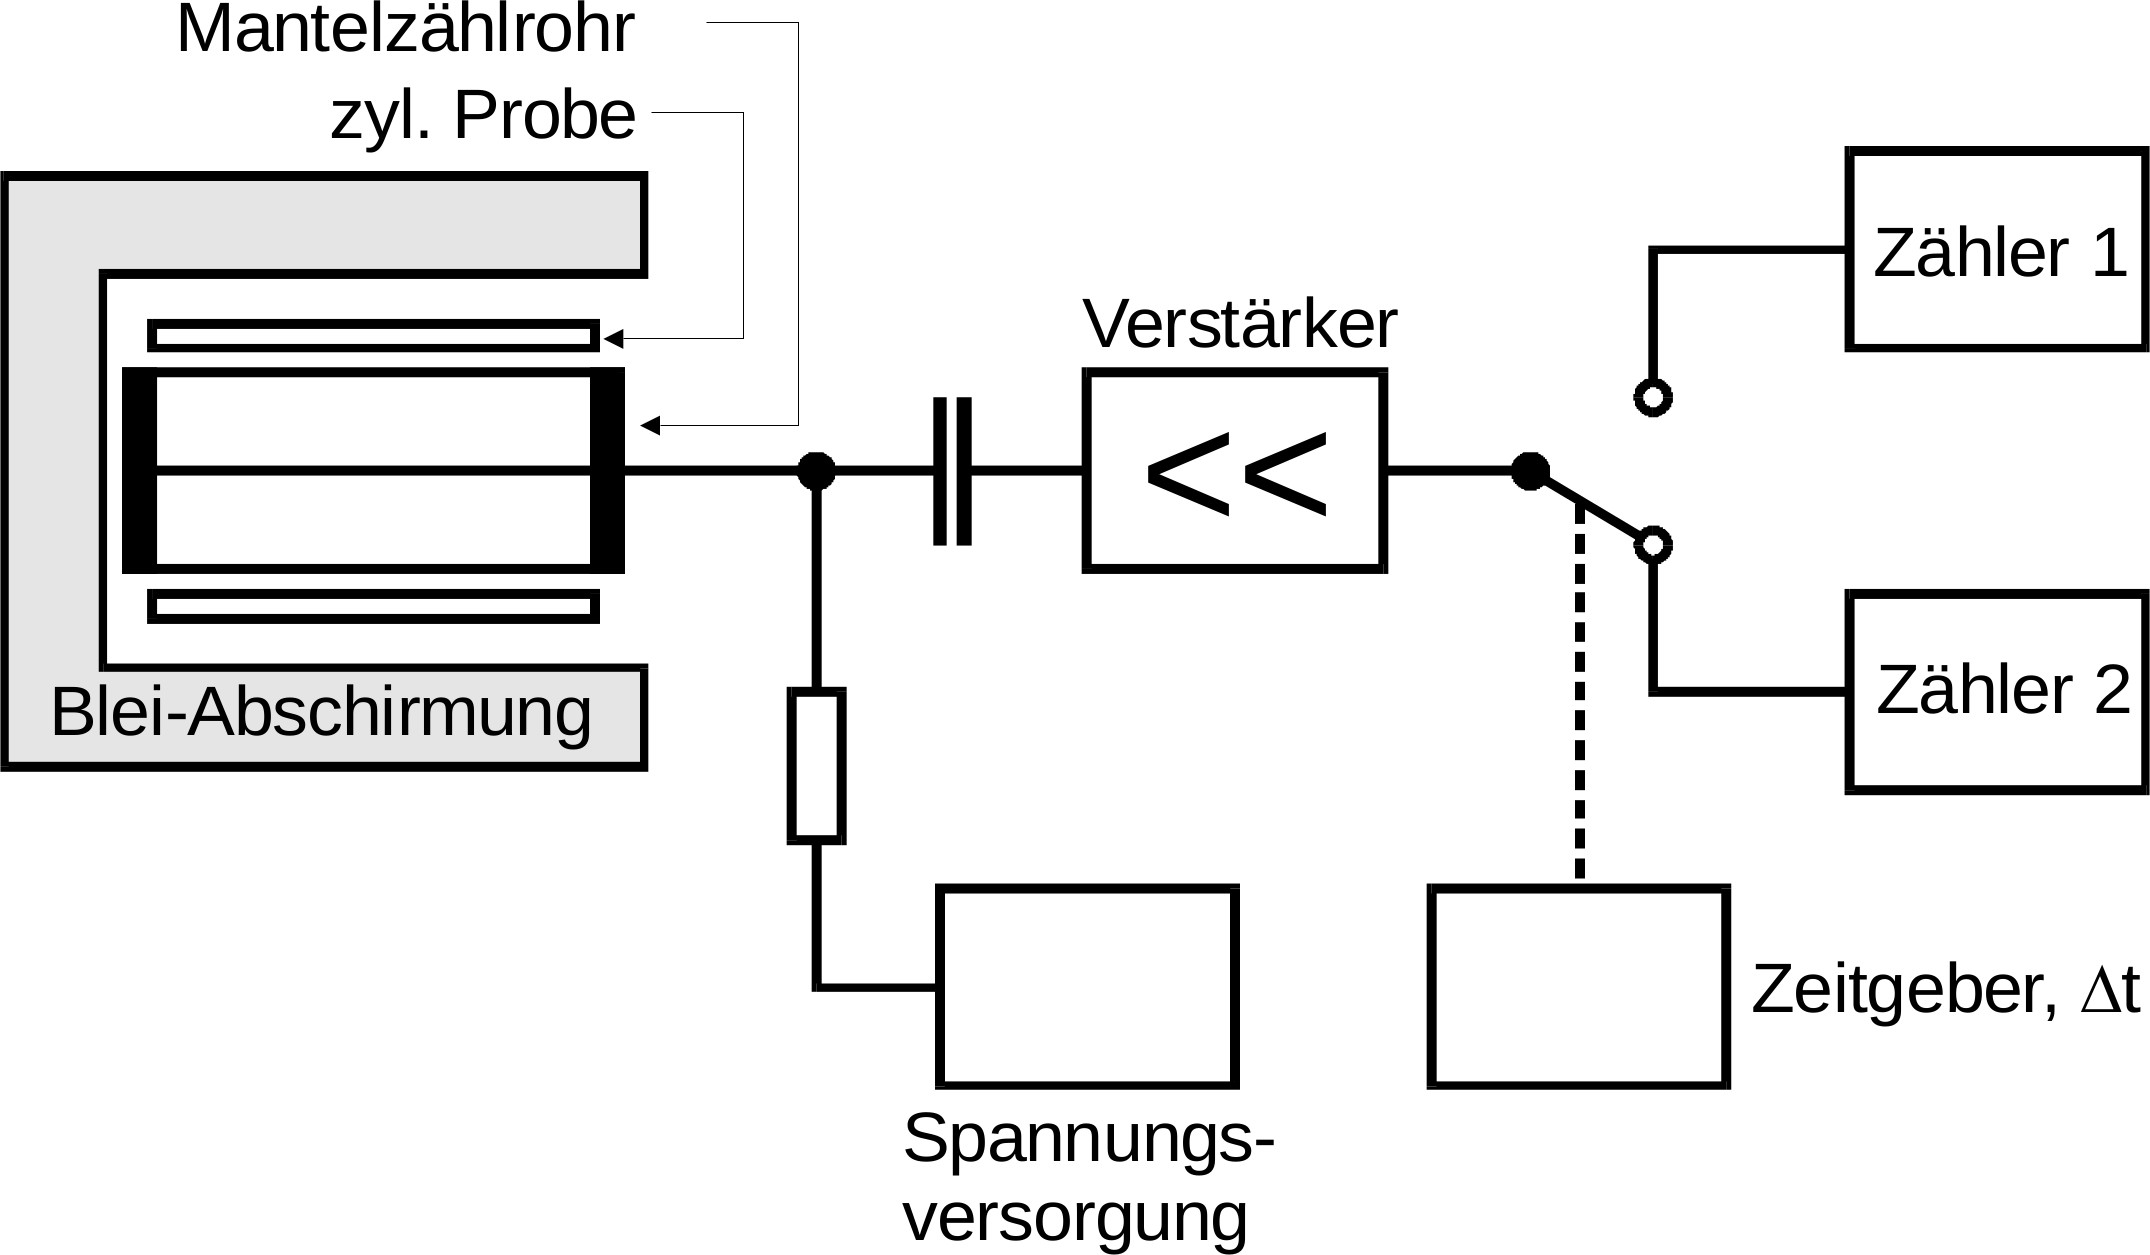
\includegraphics[width=\textwidth]{content/img/V702_Abb3.jpg}
      \caption{Schematische Darstellung des Versuchsaufbaus \cite{versuchsanleitung}.}
      \label{fig:gmz}
    \end{figure}

    Beim Zerfall der Proben entstehen $\beta^{-}$- und $\gamma$-Teilchen,
    welche mit einem Geiger-Müller-Zählrohr gemessen werden können.
    Diese Teilchen lösen im Inneren des Zählrohrs elektrische Impulse aus,
    welche zu einem elektrischen Zählwerk geleitet werden.
    Dieses misst über einen Zeitraum von $\symup{\Delta} t$
    und schaltet in einer Zeit von $\SI{100}{\nano\second}$ auf ein weiteres Zählwerk um,
    welches nach einem weiteren Zeitraum $\symup{\Delta} t$ zurück zum ersten Zählwerk umschaltet,
    sodass über einen sehr langen Zeitraum genau gemessen und bequem abgelesen werden kann.\\
    Das Geiger-Müller-Zählrohr ist von einem Block aus Blei umgeben,
    welcher den Einfluss von Höhenstrahlung und natürlicher Radioaktivität minimieren soll.
    Die endliche Zählrate,
    die trotzdem schon vor dem Einfügen der Probe gemessen wird,
    wird Nulleffekt $N_\text{U}$ genannt.
    Um diesen besonders genau zu bestimmen,
    wird vor Einfügen der Probe über einen möglichst langen Zeitraum gemessen.\\
    Für die Zählrate ergibt sich
    \begin{equation}
        \label{eqn:deltazählrate}
        N_{\symup{\Delta}t}(t_\text{i}) = N_{\symup{\Delta}t, \text{gem}}(t_\text{i}) - N_{\symup{\Delta}t, \text{u}} \; ,
    \end{equation}
    mit der über $\symup{\Delta} t$ gemessenen Zählrate $N_{\symup{\Delta}t, \text{gem}}$ und der
    Zählrate des Nulleffekts $N_{\symup{\Delta}t, \text{u}}$.
